\subsection{Does Recovery Increase Source Separation?}
\label{sec:recovery-control}

A separate physical control tests this possibility without changing the
stream method. We solve 38 complete F01 trajectories of 8 s with 241 PMU
reports each. A prior 8\% load change at bus 7 or 24 is applied at 2 s and
restored at 3 s. A weak 0.06\% load change follows after 0.5 or 2 s.
The candidate pairs are 18/27, 16/21 and 3/21, and the observation horizon
is 1.5 s. Controls and prior-severity differences account for the remaining
trajectories. Within each matched history, the secondary-event and
no-secondary-event trajectories share the same prefix. Physical and
instrumental states are retained through restoration.

This is an oracle component test: the prior trajectory, secondary onset,
load family and candidate pair are supplied. Finite-amplitude differences
of nonlinear trajectories provide incremental responses; these are
secants, not newly derived analytical tangents. The 47-coordinate F01
measurement operator is followed by its frozen innovations transform.
For a geometric control, we profile nonnegative competing amplitudes.
Adding a rank-one covariance from uncertainty of 0.01 in the previous load
fraction tests sensitivity to a nuisance direction; it is not a causal
posterior over the full state.

\begin{figure*}[t]\centering
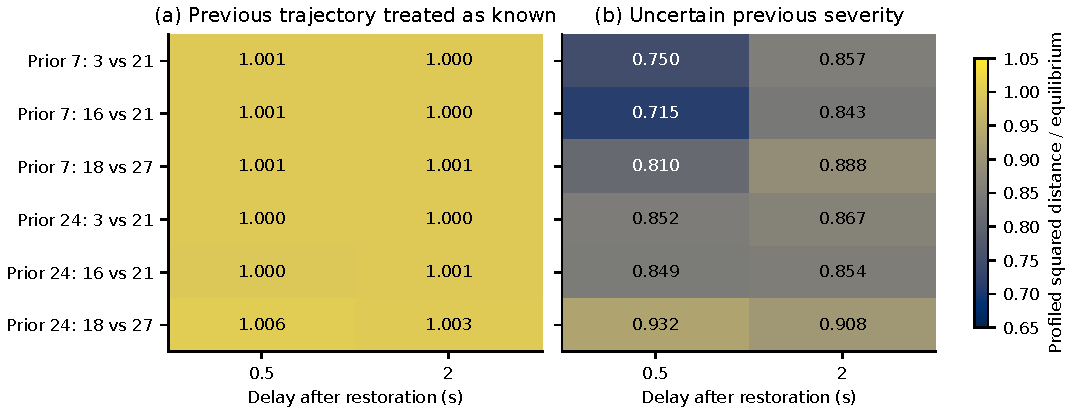
\includegraphics[width=0.98\textwidth]{figures/generated/recovery_x04_information.pdf}
\caption{Full-F01 physical control, not an R11 performance comparison.
Each cell is the profiled squared separation during recovery divided by
its equilibrium value. The same source pairs are evaluated with the
previous trajectory treated as known (left) and with one uncertain
previous-severity direction (right). Values below one mean less separation.
Adding nuisance covariance reduces precision at fixed signatures by
construction; the left panel separately shows the small change in
physical response geometry. The 12 cells share four recovery histories.}
\label{fig:recovery-x04}\end{figure*}

The median ratio is 1.0006 with known history and 0.8532 with that nuisance
direction; none of the 12 latter ratios exceeds one
(Fig.~\ref{fig:recovery-x04}). An illustrative binary likelihood comparison,
using a signed Gaussian amplitude prior of standard deviation 0.0015 and
300 common Gaussian innovation draws per generating source, gives the
same mean accuracy, 98.35\%, for equilibrium and conditioned signatures.
Two cells worsen and one improves. This likelihood experiment integrates
signed amplitudes, whereas the distance profiles nonnegative amplitudes;
the distance is not asserted to bound its error. The noise assumption is
an innovations-domain control, not validation of the complete instrumental
generator. These correlated, known-onset comparisons establish neither
an R11 improvement nor general equivalence. They provide no support for
claiming that recovery universally creates useful source information.
